%% This is file `jcomp-template.tex',
%% 
%% Copyright 2017 Elsevier Ltd
%% 
%% This file is part of the 'Elsarticle Bundle'.
%% ---------------------------------------------
%% 
%% It may be distributed under the conditions of the LaTeX Project Public
%% License, either version 1.2 of this license or (at your option) any
%% later version.  The latest version of this license is in
%%    http://www.latex-project.org/lppl.txt
%% and version 1.2 or later is part of all distributions of LaTeX
%% version 1999/12/01 or later.
%% 
%% The list of all files belonging to the 'Elsarticle Bundle' is
%% given in the file `manifest.txt'.
%% 
%% Template article for Elsevier's document class `elsarticle'
%% with harvard style bibliographic references
%%
%% $Id: jcomp-template.tex 100 2017-07-14 13:15:12Z rishi $
%%
%% Use the option review to obtain double line spacing
%\documentclass[times,review,preprint,authoryear]{elsarticle}

%% Use the options `twocolumn,final' to obtain the final layout
%% Use longtitle option to break abstract to multiple pages if overfull.
%% For Review pdf (With double line spacing)
\documentclass[times,twocolumn,final]{elsarticle}
%% For abstracts longer than one page.
%\documentclass[times,twocolumn,review,longtitle]{elsarticle}
%% For Review pdf without preprint line
%\documentclass[times,twocolumn,review,nopreprintline]{elsarticle}
%% Final pdf
%\documentclass[times,final]{elsarticle}
%%
%\documentclass[times,twocolumn,final,longtitle]{elsarticle}
%%


%% Stylefile to load JCOMP template
\usepackage{jcomp}
\usepackage{framed,multirow}
\usepackage{amsmath}
%% The amssymb package provides various useful mathematical symbols
\usepackage{amssymb}
\usepackage{latexsym}

% Following three lines are needed for this document.
% If you are not loading colors or url, then these are
% not required.
\usepackage{url}
\usepackage{xcolor}
\definecolor{newcolor}{rgb}{.8,.349,.1}

\journal{Computer Methods and Programs in Biomedicine}

\begin{document}

\verso{Anahita A. Seresti \textit{et al}}

\begin{frontmatter}

\title{Contrast Dispersion Title \tnoteref{tnote1}}%


\author[1]{Anahita \snm{A. Seresti}}

\author[2]{M. Owais \snm{Khan}\corref{cor1}}
\cortext[cor1]{Corresponding author: Department of Electrical, Computer and Biomedical Engineering, Toronto Metropolitan University, Toronto, 350 Victoria Street, Toronto, Ontario, M5B 2K3, Canada; Email: owaiskhan@torontomu.ca }


\address[1]{Department of Electrical, Computer and Biomedical Engineering, Toronto Metropolitan University, 350 Victoria Street, Toronto, M5B 0A1, Canada}


\received{1 May 2013}
\finalform{10 May 2013}
\accepted{13 May 2013}
\availableonline{15 May 2013}
%\communicated{S. Sarkar}


\begin{abstract}
%%%
\textbf{Background and Objectives}: Physics-informed neural networks (PINNs) can be used to inversely model complex physical systems by encoding the governing partial differential equations and training data into the neural network. However, neural networks are known to be biased towards learning less complex functions, called spectral bias. This has important implications in cardiovascular flows, where spatial frequencies can vary drastically across anatomies and pathologies (e.g., aneurysms or stenoses). In this study, we explore the performance of a recently-proposed Fourier-based activation function against conventional activation functions in spatially-complex patient-specific blood flow applications.

\textbf{Methods}: We evaluated the performance of $sin$ activation function against $tanh$ and $swish$ activation functions in 1D advection-diffusion problem, an eccentric 2D stenosis model (Re=5000), and a patient-specific 3D aortic model (Re=823) under pulsatile flow conditions. CFD simulations were performed at high-resolution and data points were extracted for training the neural network. We non-dimensionalized the number of training data points by $L/D$. The performance of the PINNs framework was evaluated with increasing number of trainning data points and across all three activation functions. 

\textbf{Results}: Our results demonstrate that $sine$ activation function has key desirable characteristics, such as monotonic reduction in errors,  relatively faster convergence, and accurate eigen spectra at higher modes, compared to $tanh$ and $swish$ activation functions. Interestingly, for all activation functions, the domain-averaged errors tended to asymptote at $\approx 20\%$ despite two- and four-fold increase in sensor point density. For 2D eccentric stenosis, errors asymptoted at a sensor point density of $16L/D$ while $tanh$ and $swish$ asymptoted at $24L/D$. For 3D patient-specific aorta, this asymptote was achieved at $80L/D$ for all three activation functions. 

\textbf{Conclusions}: We have demonstrated that Fourier based activation functions has higher performance in terms of accuracy and convergence properties for cardiovascular flow applications and spectral bias can limit the convergence to $\approx 20\%$ despite substantial increase in trainning data.
%%%%
\end{abstract}


\begin{keyword}
% MSC codes here, in the form: \MSC code \sep code
% or \MSC[2008] code \sep code (2000 is the default)
% Keywords
\KWD PINNs \sep Activation Functions\sep Cardiovascular Flows\sep Spectral Bias
\end{keyword}

\end{frontmatter}

%\linenumbers

%% main text

 %--------------------------------------- Introduction -----------------------------------------

\section{Introduction}
Physics-Informed Neural Networks (PINNs) have emerged as a powerful technique to encode governing partial differential equations (PDEs) and training data to model complex engineering problems. One interesting application of PINNs includes inverse solutions to the Navier-Stokes equations, which has recently been used to model blood flow in the cardiovascular system \citep{Arzani2021_PINNs, Moser2023_PINNs}. Additional losses from trainning data, obtained from experimental measurements or in-vivo imaging, can be added to the loss function to further regularize the minimization procedure in training of the neural networks. 

Vascular blood flow has conventionally been modeled via computational fluid dynamic (CFD) simulation, typically using finite element or finite volume-based methods. However, PINNs offer certain advantages over CFD that make PINNs an attractive alternative. For example, CFD relies on discretized geometries, which can be challenging to generate for complex and dynamic anatomical structures, such as heart valves and cardiac chambers {\citep{Mittal2016_Review}.  In contrast, PINNs can work on randomly-sampled points within the domain and without any need to generate conformal, discretized meshes. Another key advantage of PINNs is its ability to seamlessly integrate multi-fidelity and multi-modality data into the optimization process while CFD requires prohibitively-expensive solutions to adjoint equations to solve inverse problems. 

In recent years, PINNs have been used to model cardiovascular blood flow, such as in cerebral aneurysms and stenosed arteries. Raissi et al. were the first to demonstrate that velocity profiles in cerebral aneurysms could be reconstructed using passive scalar, albeit their findings relied on densely-defined concentration field \citep{Raissi2020_PINNs}. Building on Raissi et al.'s work, Arzani et al. demonstrated that partial measurements away from the vascular wall could be utilized to resolve near-wall hemodynamics, such as wall shear stresses, without complete information of boundary conditions \citep{Arzani2021_PINNs}. However, their findings were limited to steady flow and idealized rather than patient-specific geometries. More recently, Moser et al. evaluated the performance of various PINNs architectures in cylindrical, bifurcation and patient-specific cerebral aneurysm models \citep{Moser2023_PINNs}. One interesting observation by those authors was that patient-specific cerebral aneurysm had lower performance compared to idealized geometries, such as cylinder and bifurcation models, highlighting a frequently observed weakness of fully-connected neural networks: the spectral bias.

Spectral bias in neural networks, including PINNs, means that training process tends to learn less complex functions first \citep{Rahman2019_PINNs}. For example, the learning speed is much higher for low-frequency data but increases substantially for higher-frequency data. While various modifications to fully-connected neural networks have been proposed previously, for example by transferring the input parameters to higher parameter Fourier space, their performance in cardiovascular blood flow applications have been sub-optimal. For example, Moser et al. demonstrated that out of seven PINNs architectures tested in their study, Fourier-based PINN's had the poorest accuracy and the second highest computational cost \citep{Moser2023_PINNs}. This is a critical issue since cardiovascular blood flow can be highly dynamical, containing both low and high spatial frequencies during a cardiac cycle. Thus, robust PINNs-based approaches are needed that can minimize spectral bias. 

In this study, we propose to use Fourier-based activation functions, dubbed Sinusoidal Representation Networks ($SIREN$), which have shown to be highly effective in representing complex natural signals and their derivatives \citep{Sitzmann2020_PINNs, Pan2022_PINNs}. $SIREN$ has certain desirable properties that make it an effective choice for solving elliptical partial differential equations, such as the Navier-Stokes equations. Firstly, the derivative of a sine function is a cosine, and thus the derivative inherits the properties of the original function, enabling us to supervise complicated flow patterns that can arise in cardiovascular flows. Secondly, $sine$ activation functions converge much faster than conventional activation functions (e.g., ReLU) and thus, can reduce computational cost. A corollary to this computational advantage is the ability to minimize spectral bias and capture higher-frequency data with fewer training iterations. Despite these notable advantages, $sine$ activation functions have not yet been applied to cardiovascular blood flow applications at practical Reynolds number, such as in stenosis or aortic geometries. In this study, we will demonstrate that $sine$ activation functions offers a significant advantage over conventional activation functions, such as $tanh$ and $swish$, which are prevalent in the field of cardiovascular hemodynamics. 

%--------------------------------------- METHODOLOGY -----------------------------------------
\section{Methods}

%------------- Problem Statement ----------------------
\subsection{Problem Statement}
Here, we introduce the general form of a time-dependent PDE, given by:

\begin{equation}
\mathcal{N}(u(\textbf{x},t)) =  f(\textbf{x},t), \quad  (\textbf{x},t) \in \Omega \times [0,T]
\end{equation}
\begin{equation}
u(\textbf{x},t) =  g(\textbf{x},t), \quad \quad \quad  (\textbf{x},t) \in \partial \Omega \times [0,T]
\end{equation}
\begin{equation}
u(\textbf{x},0) =  h(x), \quad \quad \quad \quad \textbf{x} \in \Omega 
\end{equation}

where $\mathcal{N(.)}$ is the differential operation, $u$ is the solution to the PDE, and $f(\textbf{x},t)$ is the forcing term. Specifically, we are interested in the Navier-Stokes equation, which has the following form:

\begin{equation}
\dot{u} +  \textbf{u}.\nabla \textbf{u} + \frac{1}{\rho} \nabla p - \mu \nabla^{2} \textbf{u}
\end{equation}

\begin{equation}
\nabla \dot {\textbf{u}} = 0
\end{equation}

where $u(\textbf{x},t)$ is the time-dependent velocity vector field, $p(\textbf{x},t)$ is the pressure field, $\textbf{x} \in \Omega$ are the spatial coordinates, $\rho$ is the density of blood, $\nu$ is the dynamic viscosity. The boundary conditions, $\mathcal{B}$, is defined as:
\begin{equation}
\mathcal{B}(\textbf{x},t,\textbf{u},p)=0, \quad \quad \quad \textbf{x} \in \partial \Omega
\end{equation}

However, in cardiovascular flow modeling, boundary conditions are only partially known, usually on the wall of the geometry as a no-slip condition (i.e., $\textbf{u}_{wall}=0$). In addition, the inlet and outlet boundary conditions are rarely known beforehand and thus, the problem becomes ill-posed. In some situations, partial sparse measurements are known that follow the governing equations, and thus, can be incorporated into the neural network training process. 

%---------------- Physics Informed Neural network ------------------------
\subsection{Physics-informed Neural Network}
The solution, $u(\textbf{x},t)$, was approximated using a fully-connected neural network, $u(\textbf{x},t;\theta)$, where $\textbf{x}$ represents the spatial coordinates, $t$ represents time, and $\theta$ represents the trainable parameters of the deep neural network \citep{Jin2021_PINNs}. The network is defined as:

\begin{equation}
\Phi = \textbf{W}_{n}(\phi_{n-1} \circ \phi_{n-2} \circ ... \circ \phi_{0})(x)+\textbf{b}_n
\end{equation}
\begin{equation}
\textbf{x}_{i} \longmapsto \phi_{i}(\textbf{x}_{i})=\sigma(\textbf{W}_{i}\textbf{x}_{i}+\textbf{b}_i)\\
\end{equation}

Here, $\phi_{i}:\mathbb{R}^{M_{i}} \longmapsto \mathbb{R}^{N_{i}}$ corresponds to the $i_{th}$ layer of the network. Each layer consists of the affine transform defined by the weight matrix $\textbf{W}_{i} \in \mathbb{R}^{N_{i} x M_{i}}$ and the biases $\textbf{b}_i \in \mathbb{R}^{N_{i}}$ applied on the input $\textbf{x}_{i} \in \mathbb{R}^{M_{i}}$. This is followed by applying a non-linear function, $\sigma$, to each component of the activation function. 

Three losses were used for the optimization process: i) Loss from the PDEs that governs the physics of blood flow, namely the Navier-Stokes equation ($\mathcal{L}_{phys}$); ii) loss from the partially-known boundary conditions, ($\mathcal{L}_{bc}$); and iii) loss from the sensor data that further regularizes the problem in the absence of some boundary conditions ($\mathcal{L}_{data}$). Each of the individual loss components are defined as:

\begin{equation}
\mathcal{L}_{phys}=|| \dot{u} +  \textbf{u}.\nabla \textbf{u} + \frac{1}{\rho} \nabla p - \mu \nabla^{2} \textbf{u} ||_{\Omega} + ||\nabla . \textbf{u}||_{\Omega}
\end{equation}

\begin{equation}
\mathcal{L}_{bc}=|\textbf{u}-\textbf{u}_{bc}|^2
\end{equation}

\begin {equation}
\mathcal{L}_{sensor}=|\textbf{u}-\textbf{u}_{sensor}|^2
\end{equation}

 The total loss function is defined as:

\begin{equation}
\mathcal{L}_{total}(\theta)= \mathcal{L}_{phys}(\theta) + \alpha \mathcal{L}_{bc} (\theta) + \beta \mathcal{L}_{data}(\theta),
\end{equation}

Skip connections were added to the PINN architecture to improve accuracy, speed and avoid vanishing gradient problems. The accuracy of the PINNs can be sensitive to the number of layers in the network since excessive layers can deteriorate the performance of the network. The skip connections effectively enable the network to intelligently "skip" unnecessary layers, and thus, prevents the detrimental impact of additional layers. These skip connections can allow the network to be adaptable to other flow conditions even when the optimal number of layers are unknown.

%FIGURE 0
\begin{figure*}[!t]
\centering
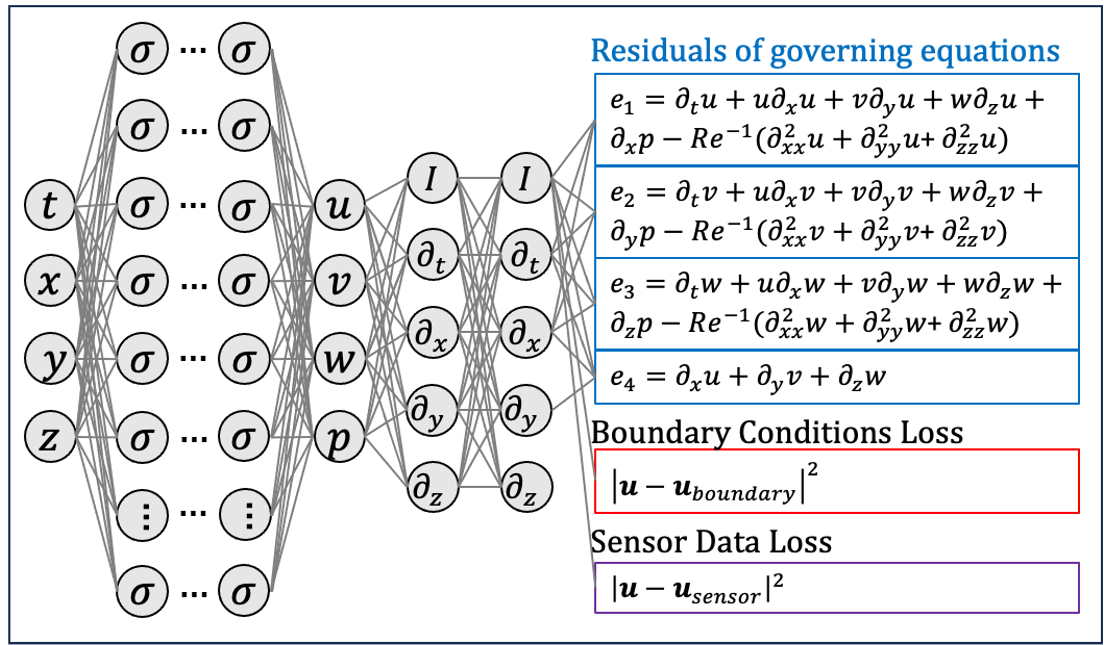
\includegraphics[width=0.8\textwidth]{./Figures/Figure_Methods_0}
\caption{A schematic of the physics-informed neural network. The left part of the neural network represents an uninformed network while the right part represents the informed network based on the physical equations (i.e., Navier-Stokes equations).}
\label{fig:Results_0}
\end{figure*}

%Adaptive Coefficients
\subsubsection{Adaptive Coefficients in the Loss Function}
The weighting coefficients in the loss equations, namely $\alpha$ and $\beta$ that determine the contribution of $\mathcal{L}_{bc}$ and $\mathcal{L}_{data}$, respectively, to the total loss, $\mathcal{L}_{total}$, and play a critical role in the training process. However, choosing these weights are typically problem-specific and thus, require tuning through a trail and error process that can be tedious and time consuming. To address this problem, we apply the strategy of dynamic weights proposed by Wang et al. \citep{Wang2020_PINNs} and adopted by Jin et al \citep{Jin2021_PINNs}. Briefly, the strategy utilizes the back-projected gradient statistics to dynamically update the coefficients during the training process. The coefficients updating process is defined as:

\begin{equation}
\begin{split}
\hat{\alpha}^{(k+1)} = \frac{ max_{\theta}\{|\nabla_\theta\mathcal{L}_{phys}|\}}{\overline{|\nabla_\theta\mathcal{L}_{bc}|}} 
\\[5pt]
\hat{\beta}^{(k+1)} = \frac{ max_{\theta}\{|\nabla_\theta\mathcal{L}_{phys}|\}}{\overline{|\nabla_\theta\mathcal{L}_{data}|}} 
\end{split}
\end{equation}

Where $\overline{|\nabla_\theta\mathcal{L}_{bc}|}$ and $\overline{|\nabla_\theta\mathcal{L}_{data}|}$ denote the mean of $|\nabla_\theta\mathcal{L}_{bc}|$ and $|\nabla_\theta\mathcal{L}_{data}|$, respectively, with respect to parameters $\theta$. To prevent abrupt alterations in the coefficients during each iteration, a moving average was employed to ensure a gradual and smooth transition, which resulted in the following equation: 

\begin{equation}
\begin{split}
\alpha^{(k+1)} = (1-\lambda)\;\alpha^{(k+1)} + \lambda\;\alpha^{(k)}
\\[5pt]
\beta^{(k+1)} = (1-\lambda)\;\beta^{(k+1)} + \lambda\;\beta^{(k)}
\end{split}
\end{equation}
Here, $\lambda$ refers to a hyperparameter, and a value of $\lambda=0.9$ was used in this study. 

\subsubsection{Activation Functions}
Activation functions play a crucial role in the neural networks enabling them to learn complex relationships between input and output data by introducing nonlinearity \citep{Jagtap2023_PINNs}. However, conventional activation functions like ReLU, Sigmoid, and $tanh$ have limitations in capturing periodicity and oscillations, which are typically observed in quasi-turbulent cardiovascular flows such as in aorta, aneurysms and cardiac chamber although they may demonstrate adequate performance under laminar flow conditions. In this study, we evaluated the performance of two conventional activation functions, namely $swish$ and $tanh$, against the SIREN architecture that uses a $sine$ activation function \citep{Sitzmann2020_PINNs}. The formulation of each of these activation functions are given below:

\begin{equation}
\text{tanh}: f(x)=\frac{e^x-e^{-x}}{e^x+e^{-x}}
\end{equation}
\begin{equation}
\text{sine}: f(x)=sin(x)
\end{equation}
\begin{equation}
\text{swish}: f(x) = x.sigmoid(x)
\end{equation}


Sinusoidal functions are well-suited to capture periodic patterns and can augment the neural network with Fourier features, significantly enhancing its ability to represent oscillatory behavior in the data. Interestingly, since the derivative of a sine function is a phase-shifted cosine, the derivative functions inherits the desirable properties of the original sine function (e.g., model high-frequency data, higher accuracy). However, sine activation functions require careful consideration during inialization to ensure proper convergence. According to Sitzmann et al., the use of periodic activation functions combined with uniformly distributed initial weights can lead to poor accuracy and convergence. Thus, a specialized initialization scheme that can preserve the distribution of activations within the neural network is required to ensure the output data is independent of the number of layers \citep{Sitzmann2020_PINNs}. The initialization scheme for the sine activation function is \citep{Pan2022_PINNs}

\begin{equation}
\theta_i \sim u\;(-\sqrt{\frac{c}{\omega_0 n}},\sqrt{\frac{c}{\omega_0 n}})
\end{equation}

Where $u$ indicates the uniform distribution, $n$ is the number of layers, and $c$ is  a hyperparameter that is assigned as $c=6$. The factor $\omega_0$ is used to increase the spatial frequency of the first layer in order to better match the frequency spectrum of the signal. A value $\omega_0=30$ is used for the first layer in 1D and 2D , $\omega_0=10$ is used for the first layer in 3D case. For the rest of the networks, $\omega_0=1$ was used. Moreover, sinusoidal activation function requires special normalization of the input components to be in the interval of $[-1 \;\; 1]$, and thus, all input parameters were normalized to be within this range. 

\subsection{Test Cases Relevant to Cardiovascular Flow Applications}
In this section, we describe three test cases that are relevant to cardiovascular blood flow applications. High-resolution CFD simulations were performed to obtain the ground truth data and subsequently used to extract sparse measurements for the training process. These sparse measurements were used to regress velocity field using PINNs with only partial boundary conditions, namely, no-slip velocity on the wall. We evaluated three activation functions, namely $sine$, $tanh$, and $swish$, all of which have previously been used in PINNs applications. We assessed the performance of these activations functions in three representative examples: i) 1D advection-diffusion equation; ii) 2D non-axisymmetric stenosis at Re=5000, and iii) 3D patient-specific aorta at Re=823. 

%----------------------- Problem 1: Advection Diffusion Equation ----------
\subsection{Test Case A: 1D Advection-Diffusion Equation}
We used PINNs to reconstruct the solution to 1D advection-diffusion equation without prescribing any boundary conditions. 1D Advection-Diffusion equation was previously used by Arzani et al. \citep{Arzani2021_PINNs} and governs several physical phenomenon relevant to cardiovascular physiology, such as mass transport in atherosclerosis and thrombosis or to model the concentration of a chemical advected by a one-dimensional flow field. Secondly, advection-diffusion equations also pose numerical challenges at high Peclet and Schmidt numbers, and thus offers a sufficiently complex problem to test the theoretical performance of different activation functions. The 1D advection-diffusion equation can be expressed as:

\begin{equation}
\alpha \frac{\partial u}{\partial x} = \nu \frac{{\partial}^2 u}{\partial x^2}
\end{equation}

where $u(x)$ is the convected velocity, $a > 0$ is the local advecting velocity,  $\nu$ is the diffusion coefficient, and $x \in [0,1]$. The analytical solution to this PDE is expressed below:

\begin{equation}
u(x)=\frac{u_2 - u_1}{e^{\frac{\alpha}{\nu}}-1} e^{\frac{\alpha}{\nu} x} + \frac{ u_{1} e^{\frac{\alpha}{\nu}} - u_2}{e^{\frac{\alpha}{\nu}-1}}
\end{equation}

Here, $u_1$ and $u_2$ are the known values at the boundaries (i.e., $x=0$ and $x=1$), $\alpha=1$ and $\nu=0.01$. We used three measurement points, two outside the boundary layer, and one within the boundary layer. The problem was solved with the PINNs approach described above without enforcing the boundary conditions, $u_1$ and $u_2$. The neural network layers were varied from 2 to 10 in increments of 2, and the learning rate was adopted from 1e-3 to 1e-6 with a step decay over 5000 epoches.

%----------------------- Problem 2: 2D Non-Axisymmetric Stenosis ----------
\subsection{Test Case B: 2D Non-Axisymmetric Stenosis at Re=5000}
We used a 2D non-axisymmetric stenosis model that has previously been used in 3D to characterize transition to turbulence in stenosed arteries \citep{Varghese2007_DNS} (see Figure ~\ref{fig:Methods_2}). While the 2D model can not sustain true turbulence, we  increased the Reynolds number to 5000 to increase the complexity of the flow patterns (e.g., periodic vortex shedding) to determine how well the three activation functions perform under highly dynamical flow conditions. The flow in this geometry destabalizes due to the slight eccentricity in the stenosis neck that acts as a geometric perturbation to the flow field, and thus, avoids the need to induce perturbations into the velocity field.  

CFD simulations were performed to obtain the ground truth data using the $Oasis$ solver \citep{Mortensen2015_CFD}. $Oasis$ is a higher-order, minimally-dissipative and energy-preserving finite-element based solver that has shown comparable accuracy to spectral element solver, especially to capture transitional and turbulent cardiovascular flows \citep{Khan2019_DNS}. A second-order polynomial function was used for velocity and a first order polynomial function was used for pressure. The geometry was meshed in 60,000 triangular elements, corresponding to ~240,000 linear triangular elements. The simulation was run for 125 non-dimensional time units, $t*=tu_i/D$, for 25,000 time-steps.

The PINNs architecture consisted of 4 layers with 128 neurons per layer. The boundary conditions and the velocity field at the mesh nodes were treated as unknown quantities. Sensitivity to sensor data obtained from the CFD simulations were evaluated by systematically increasing the number of sensor points as shown in Figure ~\ref{fig:Methods_3}. Briefly, first a single row of 25 sensor points were uniformly distributed along the centerline of the geometry. The distribution of sensor points were increased uniformly in $x$ and $y$ direction by a factor of 2, 3, 4, 5, 6 and 7. These resulted ins sensor points ranging from $25 - 1225$. Only first four sensor point distributions are shown in Figure ~\ref{fig:Methods_3}. 

%FIGURE 1
\begin{figure*}[!t]
\centering
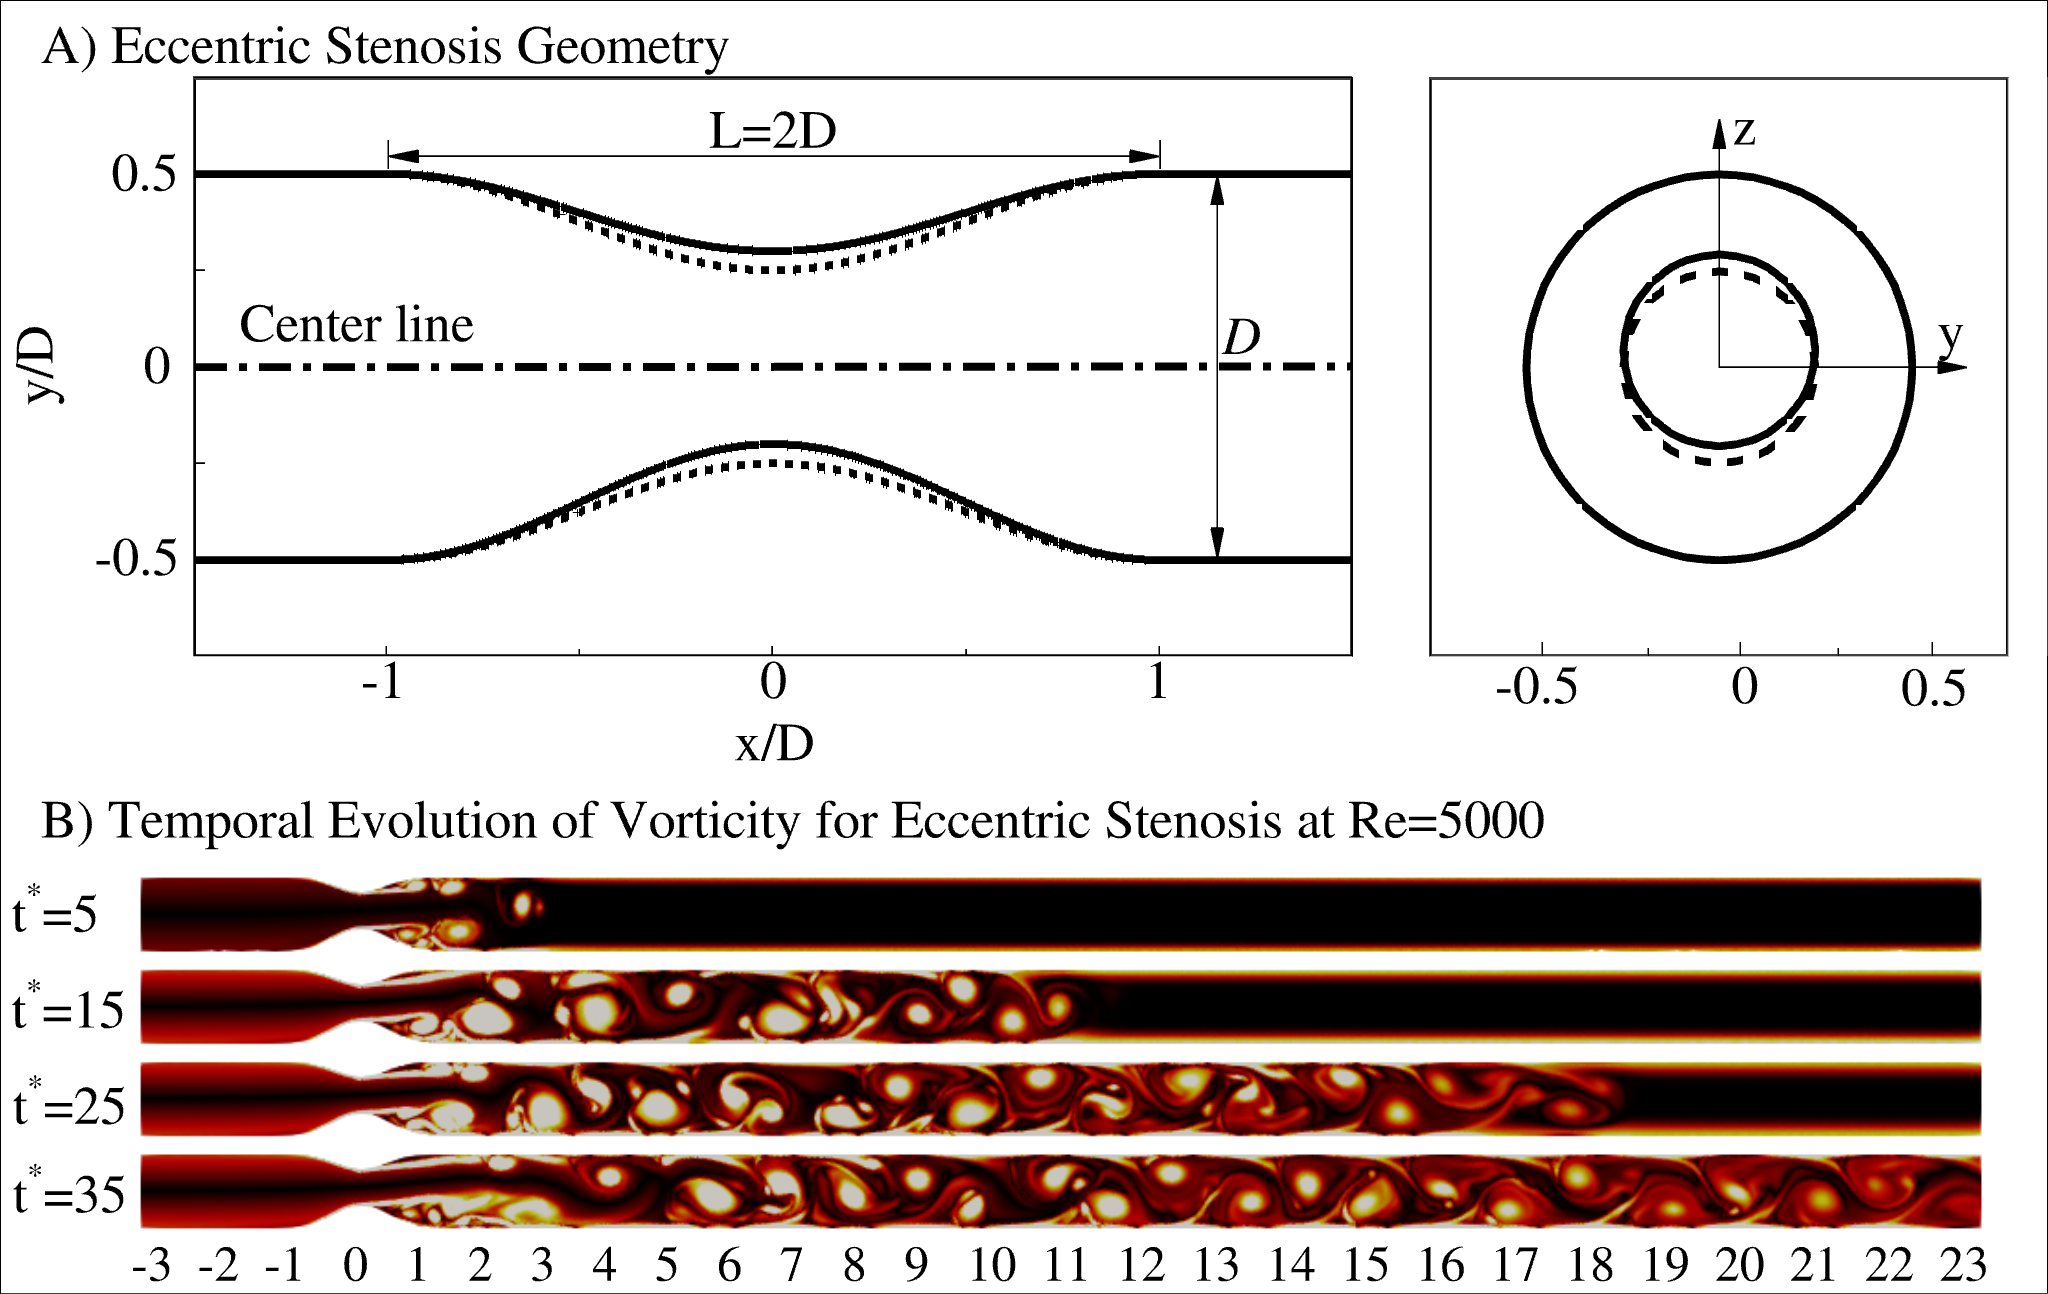
\includegraphics[width=0.95\textwidth]{./Figures/Figure1_StenosisModel}
\caption{The 2D non-axisymmetric stenosis geometry used to test the performance of the three activation functions. A) Axial and cross-sectional view of the stenotic geometry, adapted from \citep{Varghese2007_DNS}. Schematic for the axisymmetric (dashed line) and non-axisymmetric models (solid line) are shown, although only the latter was considered in the present study; $x$ corresponds to the stream-wise direction, and $y$ and $z$ correspond to the cross-stream directions. $D$ corresponds to the diameter, and $L$ corresponds to the length of the stenosis; B) Temporal evolution of vorticity at $Re=5000$. $t^{*}$ corresponds to non-dimensional time units, defined by $tu_{i}/D$. }
\label{fig:Methods_2}
\end{figure*}



%Figure 2
\begin{figure*}[!t]
\centering
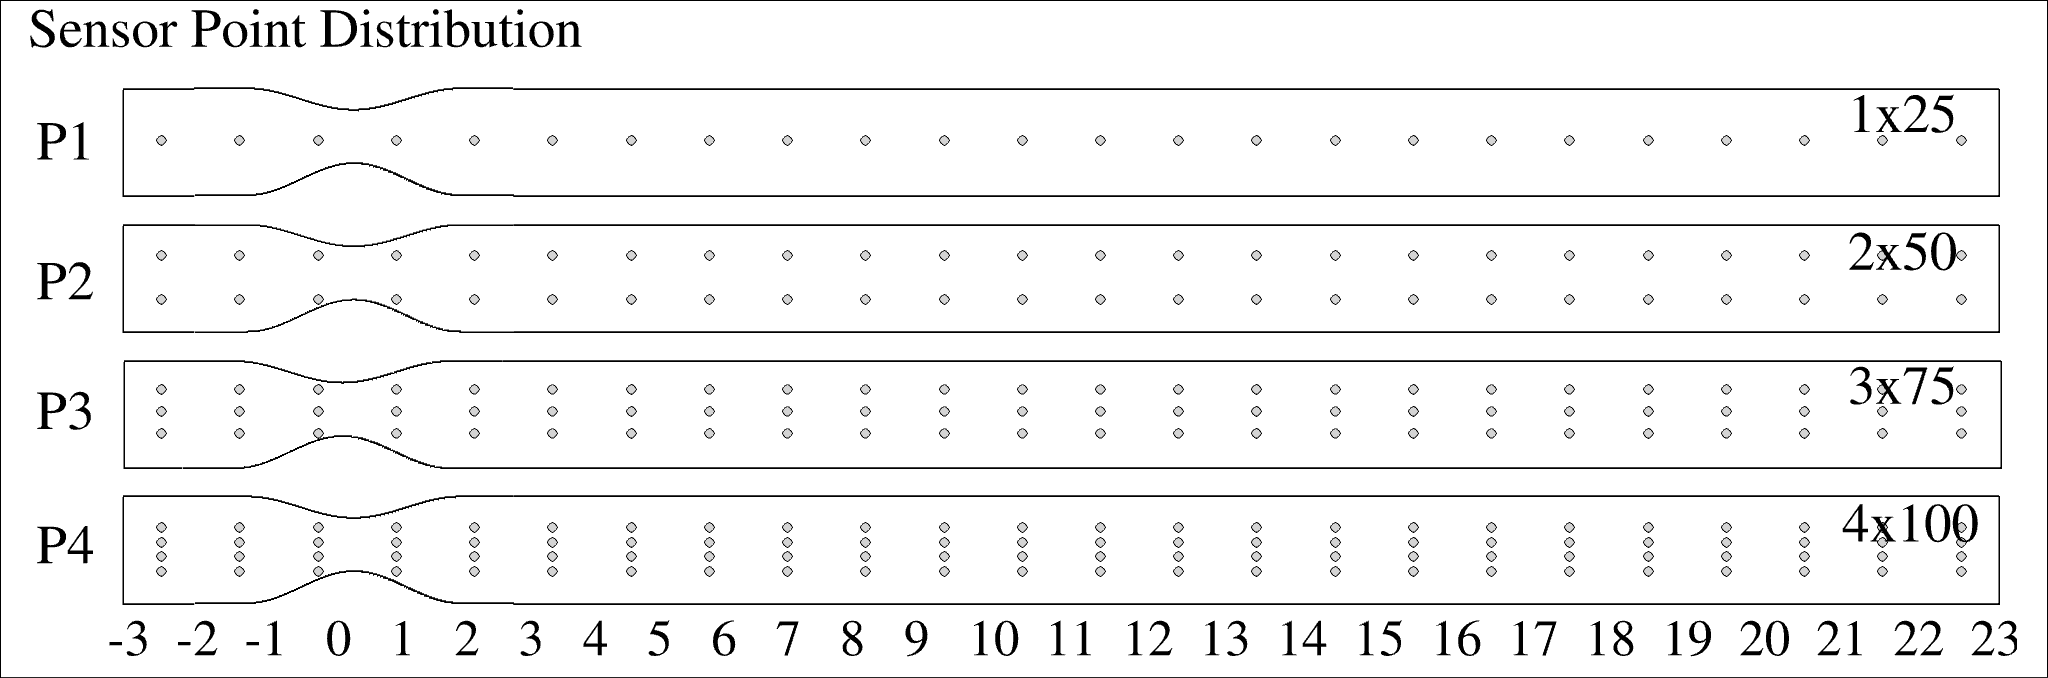
\includegraphics[width=0.95\textwidth]{./Figures/Figure2_StenosisModel_Sensors}
\caption{The distribution of known sensor points extracted from CFD simulations that were used in the loss function of the neural network. The sensor point density was increased uniformly in $x$ and $y$ directions by a factor of 2, 3, 4, 5, 6 and 7. The figure shows only the sensor point distribution of the first four cases.}
\label{fig:Methods_3}
\end{figure*}

%----------------------- Problem 3: Aortic Geometry ----------
\subsection{Test Case C: Patient-Specific 3D Aortic Geometry}
We used a 3D patient-specific aortic geometry, which can be downloaded from the open-source \textit{Vascular Model Repository} (www.vascularmodel.com, patient ID: 01750000). The aortic model is of a 45 year old male diagnosed with Marfan Syndrome. The patient had an aortic flow rate of 108mL/s, corresponding to a cycled-averaged Reynolds number of 823, and thus, may exhibit turbulent-like flow patterns at peak systolic flow conditions. The aorta was segmented and reconstructed in SimVascular and meshed into 3.2 million tetrahedral elements. Boundary conditions were assigned such that 25\% of the flow was fed to the head and neck vessels while 75\% of the flow was fed to the descending aorta. CFD simulations were run for 4 cardiac cycles with 10,000 time-steps per cardiac cycles. 

The PINNs architecture consisted of 4 layers with 128 neurons per layer. The boundary conditions and the velocity field at the mesh nodes were treated as unknown quantities. Sensitivity to sensor data obtained from the CFD simulation were evaluated by increasing the number of sensor points from 200 to 1600 points (increments of 200) equally distributed in the aortic geometry. 

%-------------------- Proper Orthogonal Decomposition -----------------
Proper Orthogonal Decomposition (POD) was used to investigate the distribution of kinetic energy over increasing Eigen modes for the three different activation functions. Given that the CFD simulation data was large, we used the method of $snapshots$, originally proposed by Sirovich et al. \citep{Sirovich1987_POD}, rather than the classical approach. For details regarding POD, readers are referred to \citep{Nobach2007_POD}. The eigenvalue problem to solve is as follows:

\begin{equation}
\int_{T}C(t,t^{'})a_{m}(t^{'}dt^{'}=\lambda_{m}a_{m}(t) 
\end{equation}

\begin{equation}
C(t,t^{'})=1/T\int_{\Omega}u_{i}(x,t)u_{i}(x,t^{'})
\end{equation}

where $C(t,t^{'})$ is the two-point temporal autocorrelation matrix, $a_{k}(t)$ and $\lambda_{k}$ are the eigenvectors and eigenvalues of $C(t,t^{'})$, respectively. Analyzing the eigenvalues can provide information regarding the distribution of kinetic energy in each mode. The modes with the lowest numbers are the most energetic modes and correspond to the coherent flow structures. The distribution of kinetic energy over modes can then be computed as $E_{M}=  \sum_{k=n}^{k=m} \lambda_{k}$.

\subsection{Standardization of Sensor Points}
Although we chose the density of sensor points heuristically, this choice can be challenging when extending our approach to different vascular territories or pathologies. Hence, it is important to standardize the sensor point density such that it is easier to compare these findings with other studies. We chose to normalized the number of sensor points by the normalized length of the vascular geometry, defined as follows:

\begin{equation}
Sensor\, Point\, Density = Total\, Number\, of\, Sensor\, Points\, . \frac{D}{L} 
\end{equation}

where $Sensor\, Point\, Density$ is the density of sensor points per normalized length of the vascular segment. $D$ and $L$ are the average diameter and the total length of the vasculature segment. 

%------------------------------------ RESULTS ------------------------------------------------
\section{Results}
%1D Advection Diffusion Equation
\subsection{Test Case A: 1D Advection Diffusion Equation}
Figure ~\ref{Figure:Results_1} shows the performance of the three activation functions, $sine$, $tanh$, and $swish$, for the 1D advection-diffusion equation. Figure ~\ref{Figure:Results_1}A  shows that the $sine$ activation function was able to reconstruct the analytical solution with only two hidden layers and with errors that were two order-of-magnitude lower than the other two activation functions. The $L_{2}$-error norms for the $sine$ activation function decreased monotonically with increasing number of layers. On the other hand, $tanh$ and $swish$ activation functions needed at least 10 hidden layers before any discernible decrease in $L_{2}$-error norms could be observed (see Figure ~\ref{Figure:Results_1}A inset). These observations are also evident from Figure ~\ref{Figure:Results_1}B, which shows convergence of mean-squared errors for $sine$ activation function with four hidden layers, while the other two activation functions required at least 10 hidden layers to show any noticeable decrease in mean squared errors. 

%Figure 3
\begin{figure*}[!t]
\centering
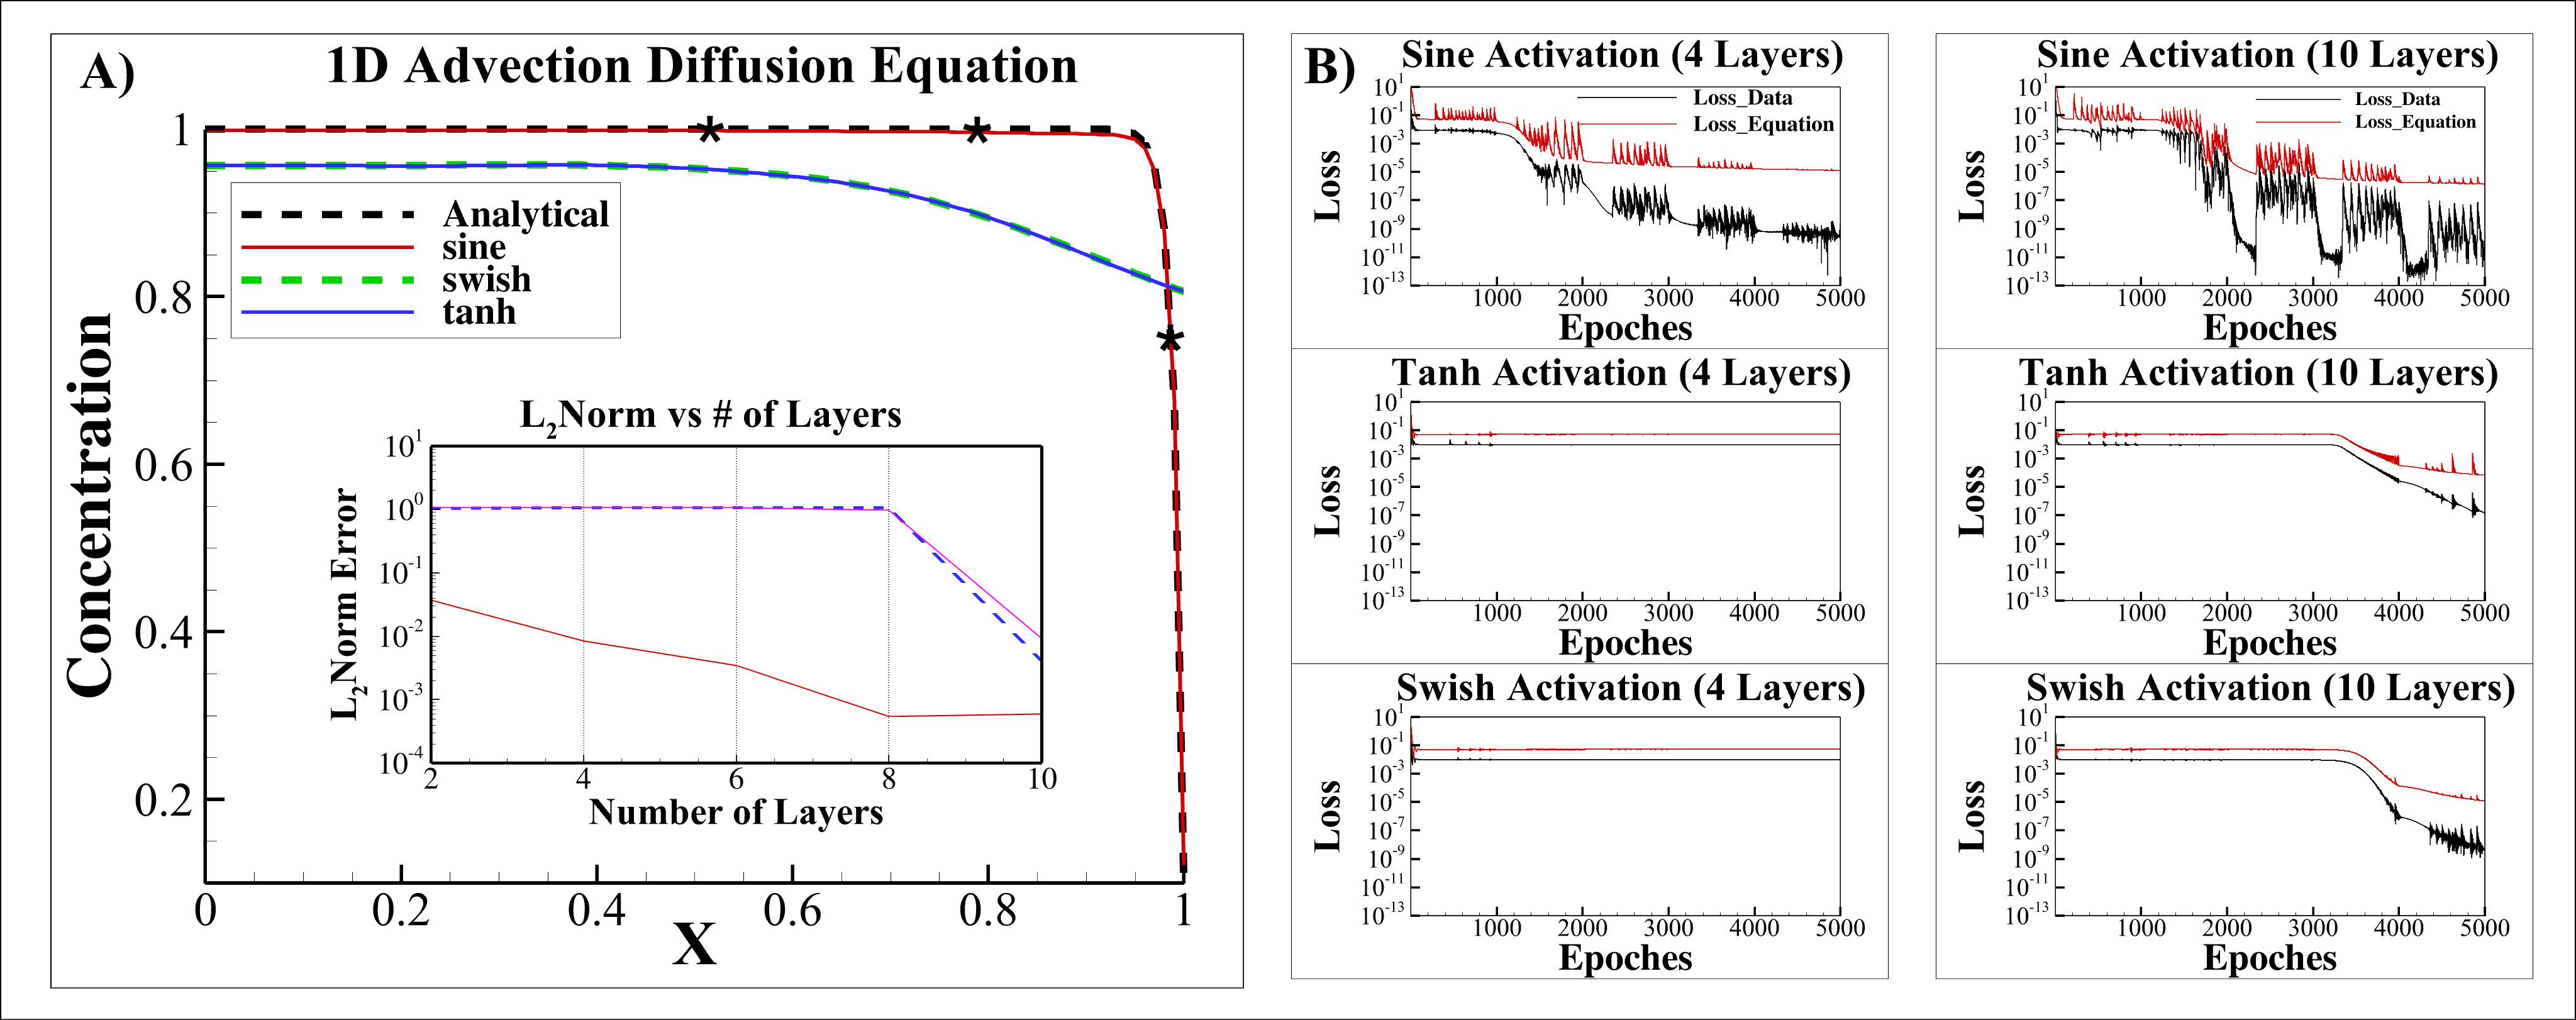
\includegraphics[width=0.95\textwidth]{./Figures/Figure3_AdvectionDiffusion}
\caption{PINN solution for $sine$, $tanh$ and $swish$ activation functions for the 1D advection diffusion equation. A) Solution to the 1D advection-diffusion equation with the three activation functions using two neural network layers. Three sensor points were used (marked with *). The inset shows the changes in $L_{2}$-error norms with increasing number of layers. B) Mean squared errors for the three activation functions with 4 layers and 10 layers.}
\label{Figure:Results_1}
\end{figure*}

%2D Non-axisymmetric Stenosis
\subsection{Test Case B: 2D Non-Axisymmetric Stenosis at Re=5000}
Figure ~\ref{fig:Results_2}A show the cross-section velocity distribution for the $sine$, $tanh$ and $swish$ activation functions with increasing number of sensor points. The $sine$ activation function was able to capture the oscillations in the flow field even with only 200 sensor points, while at least 400 points were needed to reconstruct the oscillatory flow patterns in the post-stenotic regions for $tanh$ and $swish$ activation functions. These observations are also evident from the quantitative analysis in Figure ~\ref{fig:Results_2}C, which shows that $sine$ activation function was able to converge to an error of approximately 25\% with a sensor point density of only 16 (i.e., 400 sensor points), while both $tanh$ and $swish$ activation functions needed a sensor point density of approximately 40 (i.e, 1000 sensor point) to converge to the same error levels. In addition, only $sine$ activation function showed a monotonic reduction in errors while both $tanh$ and $swish$ activation functions demonstrated a non-monotonic reduction in errors. 



%Figure 4
\begin{figure*}[!t]
\centering
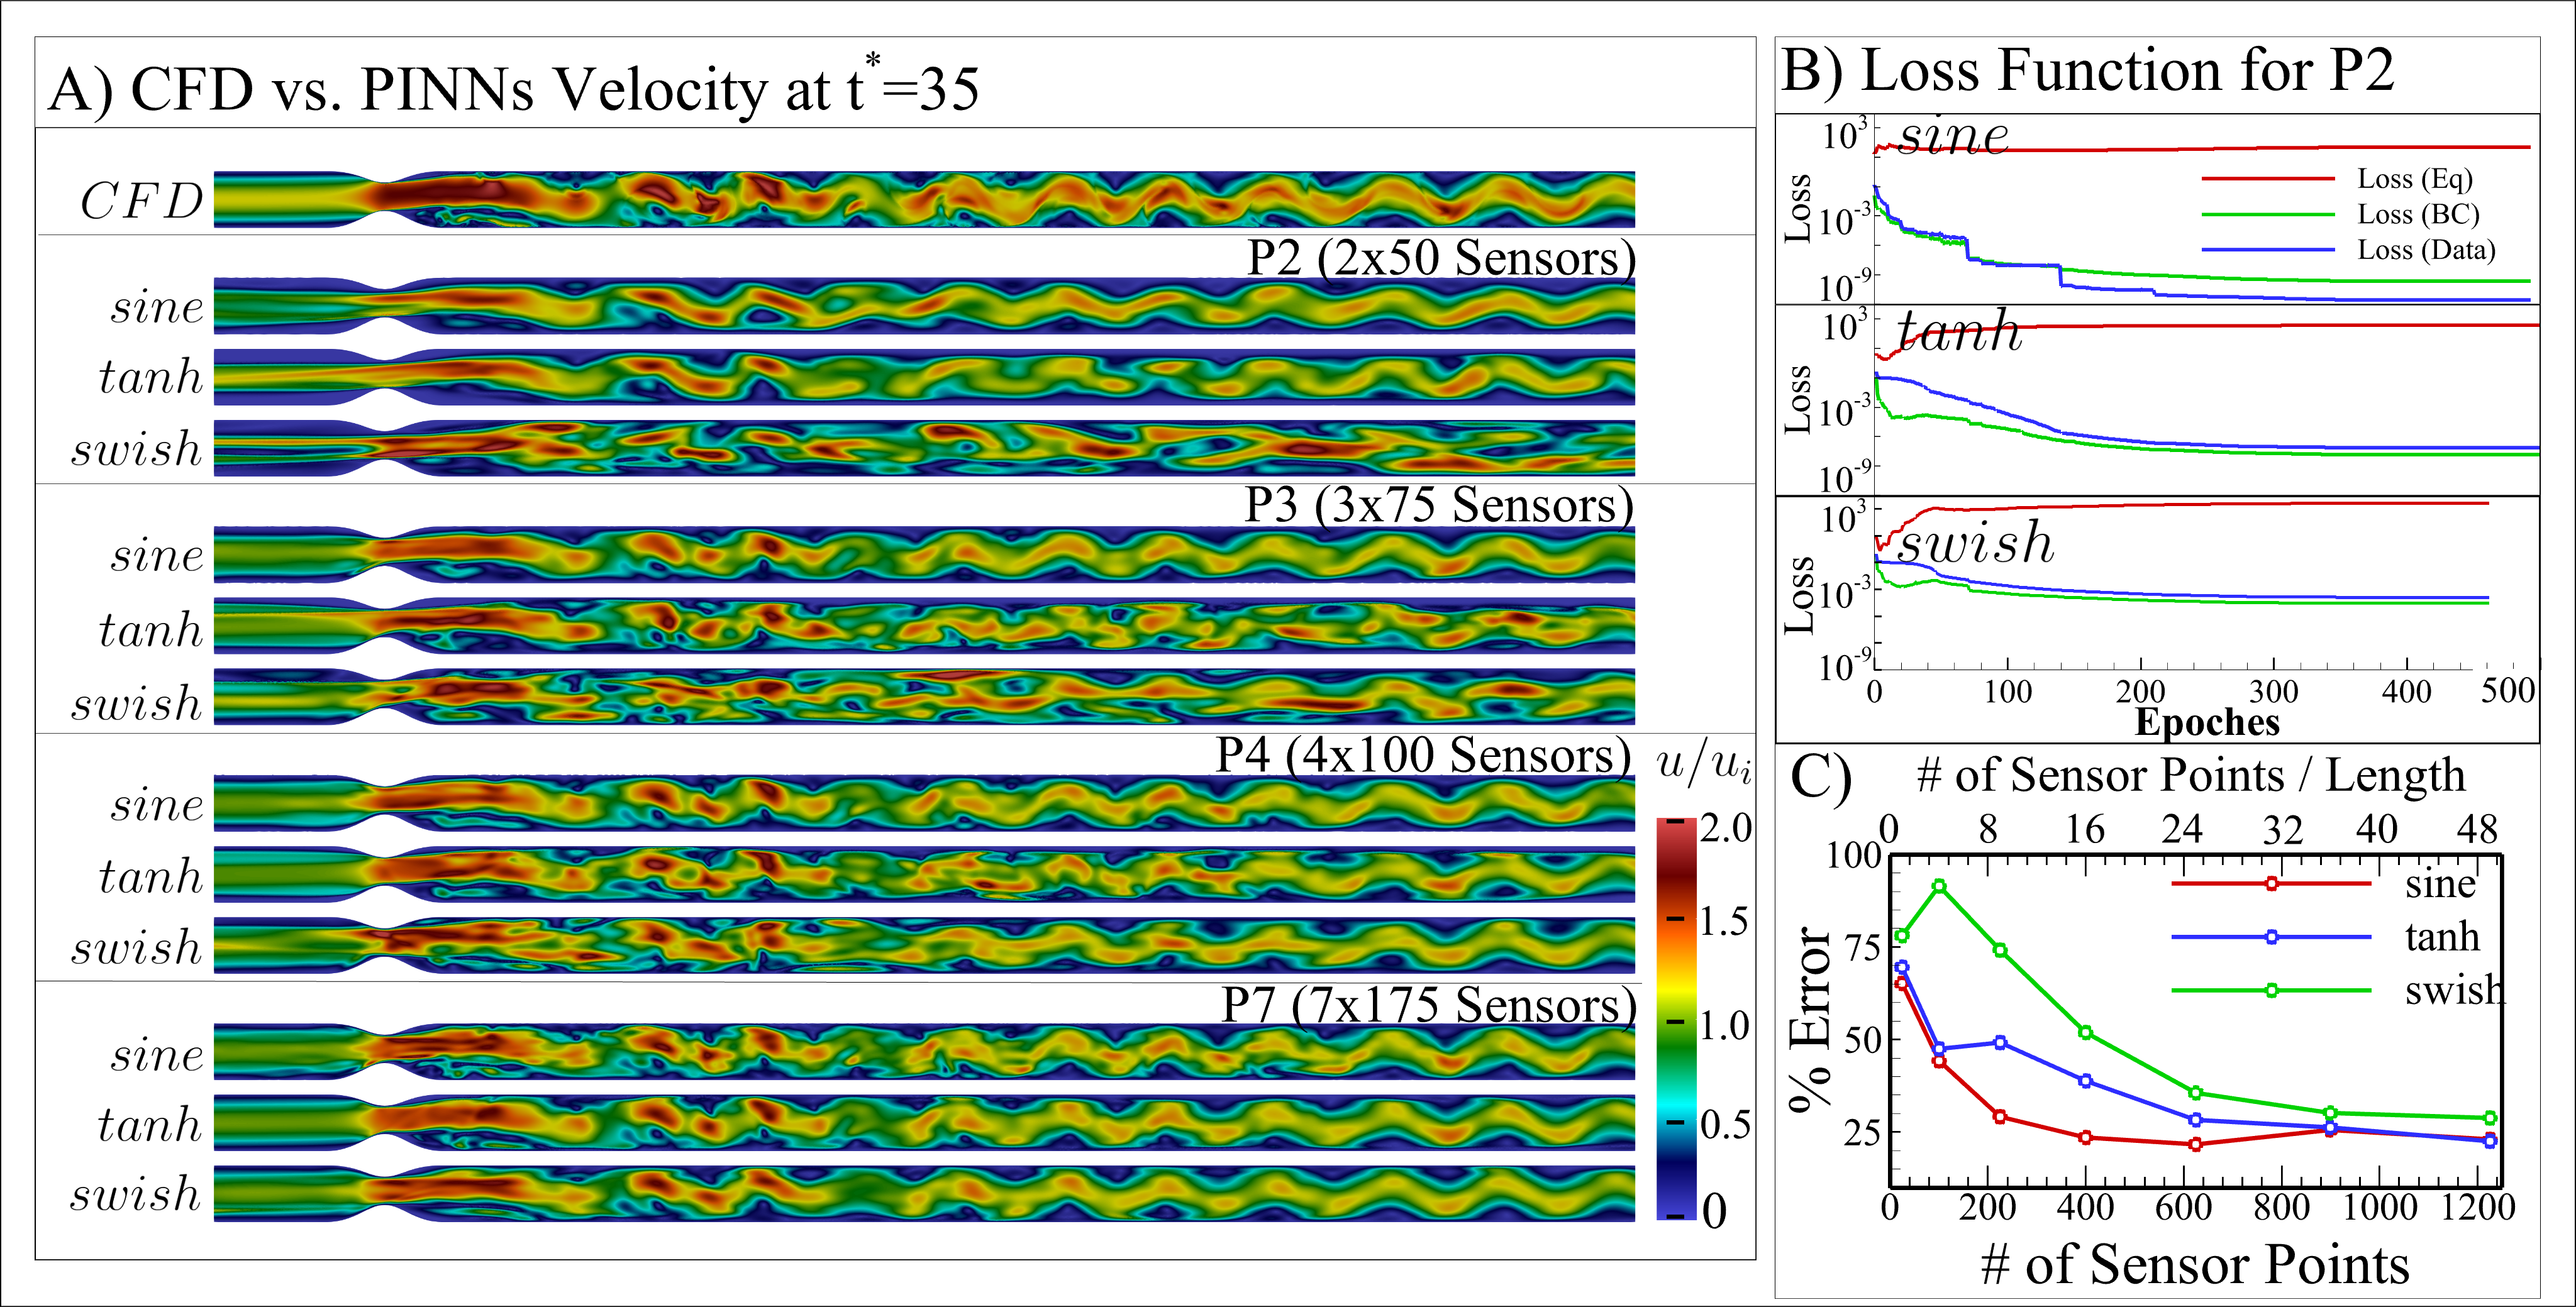
\includegraphics[width=0.95\textwidth]{./Figures/Figure4_StenosisResults_v2}
\caption{PINNs solution for $sine$, $swish$ and $tanh$ activation functions for the 2D non-axisymmetric stenosis model at non-dimensional time of $t^{*}=35$ and Reynolds number of 5000. A) Reconstructed stream-wise velocity maps with increasing number of sensor points; B) Loss functions for P2 (i.e., with 2x5 sensors); C) Percent errors for the three activation functions with increasing sensor points and sensor point density.}
\label{fig:Results_2}
\end{figure*}


%3D Aortic Geometry
\subsection{Test Case C: Patient-Specific 3D Aortic Geometry}
Figure ~\ref{fig:Results_5} shows the performance of $sine$, $tanh$, and $swish$ activation functions in a 3D patient-specific aortic geometry at peak systole. Based on the qualitative velocity maps shown in Figure ~\ref{fig:Results_5}, it can be noted that a sensor point density of 40 (i.e, 800 sensor points) was needed to reconstruct the gross flow patterns observed in the ground-truth CFD simulations. The quantitative analysis, shown in Figure ~\ref{fig:Results_5}C, demonstrates that both $sine$ and $tanh$ had similar errors, while $swish$ had comparatively higher errors for the same number of sensor data points.

POD analysis was performed to visualize the eigenspectra of the velocity field reconstructed from the three activation functions. Figure ~\ref{fig:Results_6} shows that for the case with 200 sensor points, all three activation functions showed similar Eigen spectra. However, with increasing number of sensor points, the $sine$ activation function was able to capture the energy content at higher modes much better than the other two activation functions, highlighting its ability to obtain high-frequency spatial structures in the velocity field . For example, for case with 800 sensor points and above, both $tanh$ and $swish$ activation functions were unable to adequately capture the kinetic energy in modes greater than 10. On the other hand, $sine$ activation function was able to better capture the energy content at these modes, matching well to the Eigen spectra obtained from the ground-truth CFD simulations. 

%Figure 5
\begin{figure*}[!t]
\centering
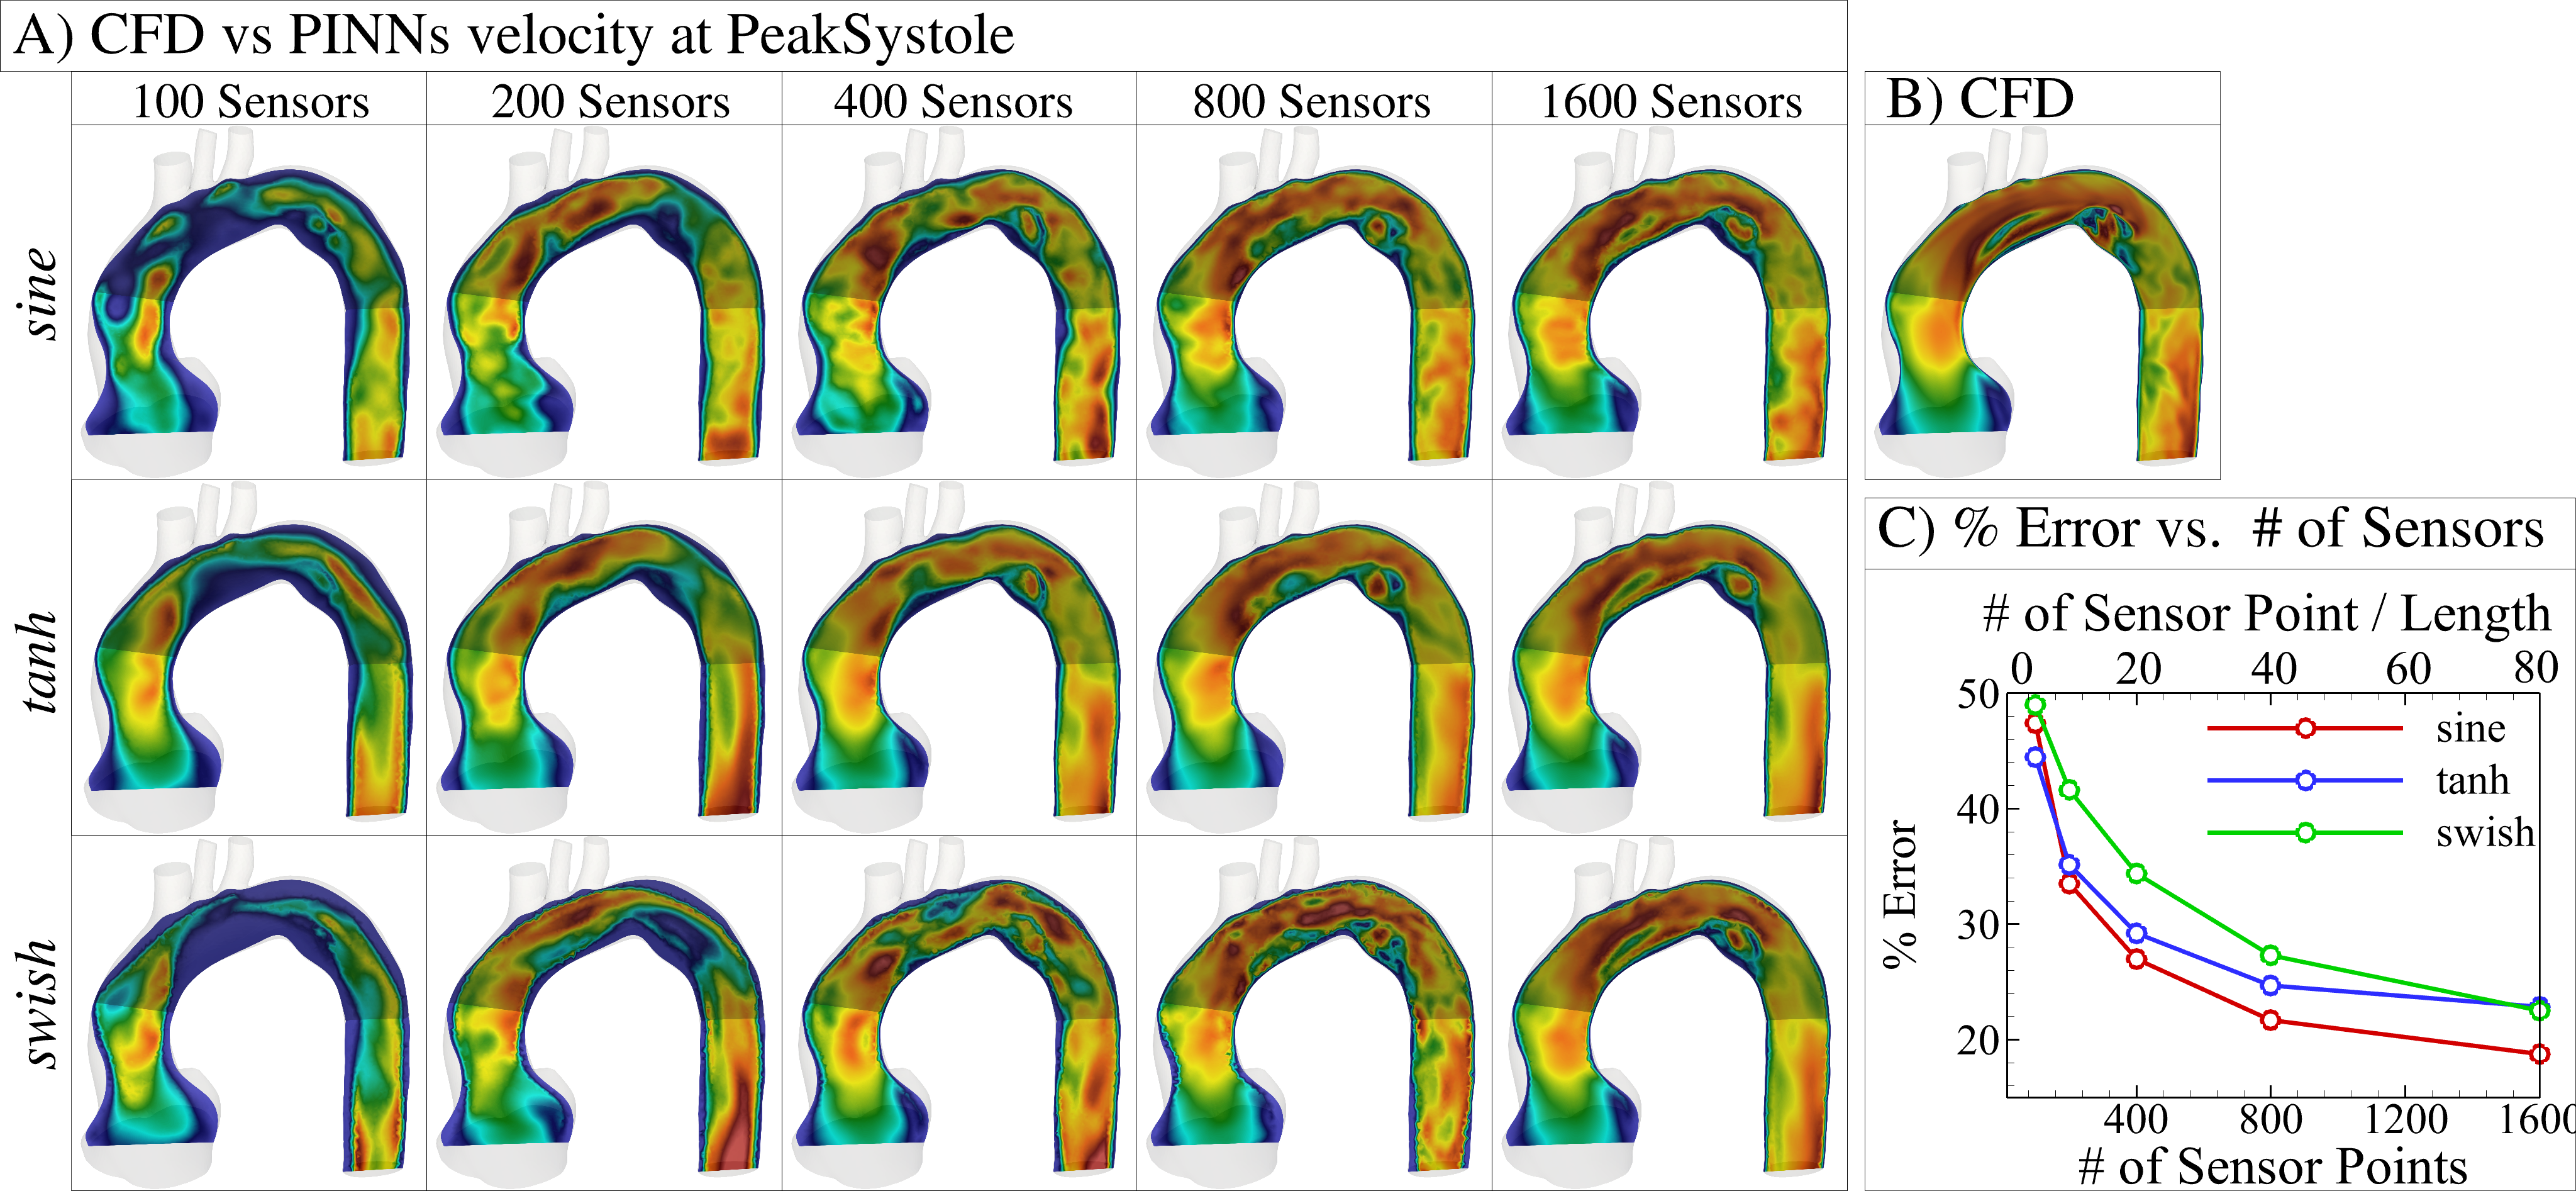
\includegraphics[width=0.95\textwidth]{./Figures/Figure5_Aorta}
\caption{PINN solution for $sine$, $swish$ and $tanh$ activation functions for the 3D patient-specific aortic model at peak systole and Reynolds number of 823. A) PINNs-derived velocity maps with increasing number of sensor points from $100-1600$ at peak systole; B) Ground-truth solution obtained from CFD simulations; C)  Percent errors for the three activation functions with increasing sensor points and sensor point density. }
\label{fig:Results_5}
\end{figure*}

%Figure 6
\begin{figure*}[!t]
\centering
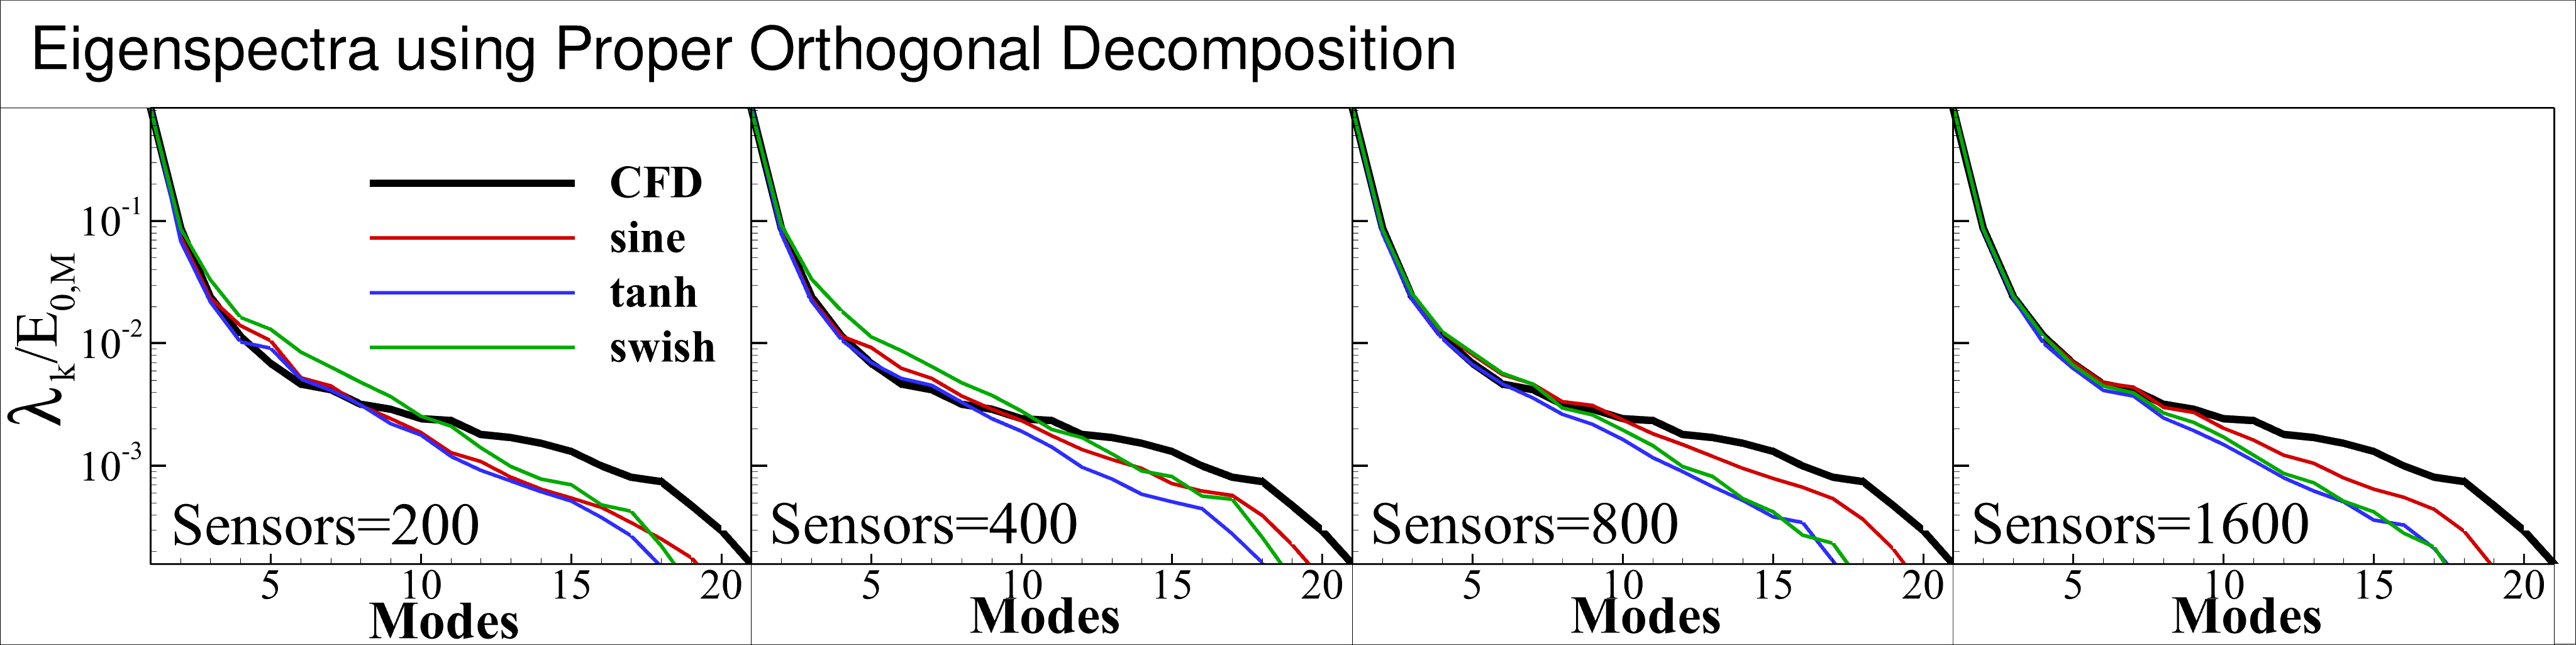
\includegraphics[width=0.95\textwidth]{./Figures/Figure6_Aorta_POD}
\caption{Eigenspectra of temporal autocorrelation derived from proper orthogonal decomposition analysis for the 3D aorta model. Eigenvalue for each mode has been normalized by the sum of all eigenvalues from modes 0 to 20.}
\label{fig:Results_6}
\end{figure*}

%%%%%%%%%%%%%%%%% DISCUSSION %%%%%%%%%%%%%%%%%%%%
\section{Discussion}
\subsection {Higher Performance of $sine$ Activation Function to Model Complex Cardiovascular Flows}
Activation functions play a key role in the training process of the neural networks and determine the overall performance and accuracy of the learned solutions. Common activation functions, such as $ReLU$, $tanh$, $swish$, and $sigmod$, have been observed and proven to suffer from substantial inefficiency on learning high-frequency functions, even with increased network complexity \citep{Tancik2020_PINNs}. The failure of standard neural networks on high-frequency functions is a well-known phenomenon, called spectral bias \citep{Rahman2019_PINNs}. These limitations of standard activation functions can be problematic in modeling complex cardiovascular flows that often contain high-frequency spatio-temporal flow fluctuations. Indeed, recent evidences from super-resolution CFD simulations and experimental measurements have shown the presence and prevalence of high-frequency spatio-temporal flow fluctuations, often termed "turbulent-like" flows \citep{Khan2021_Aneurysms,Bruneau2023_Aneurysm} . These findings raise questions regarding the applicability of PINNs, specifically with conventional activation functions, to model complex, turbulent-like cardiovascular flows. 

Our work builds on the recent developments in the field of computer vision, which have proposed remedies to learn high-frequency content with the use of Fourier features \citep{Tancik2020_PINNs} or $\omega_{0}$-scaled sine activation function \citep{Sitzmann2020_PINNs}. The former approach, which uses Fourier features, was introduced recently in the PINNs community by Wang et al. \citep{Wang2020_PINNs} but with the requirement to tune length scales of the Fourier features for each application. However, problem-specific tuning of length-scales is infeasible for cardiovascular applications, where flow conditions and geometric complexity can vary substantially depending on the anatomic location (e.g, aorta vs. cerebral vasculature) or flow conditions (e.g., aneurysm vs. stenosis). Hence, in our study, we have used the approach of Sitzmann et al., since their implementation is less sensitive to the choices of hyper-parameters of the neural network compared to the original Fourier feature approach. 

A recent study by Moser et al. compared the performance of various neural network architecture for cardiovascular flow applications \citep{Moser2023_PINNs}. Interestingly, those authors demonstrated that the modified Fourier Network architecture, as proposed by Wang et al., had the poorest accuracy amongst all architectures considered. While the reason for these negative findings are unclear, it is possible that the length scales were not tuned adequately for the problem. Instead of modifying the neural network architecture, we have used $sine$ as an activation function in the hidden layers, following the implementation of Sitzmann et al.\citep{Sitzmann2020_PINNs}, and have shown that this approach resulted in substantially higher accuracy compared to other conventional activation functions.

\subsection {Requirements on the Number of Sensor Points for Vascular Territories}
One of the key strengths of PINNs is the ability to include known sensor data, such as those measured invasively in a patient or through imaging (e.g., 4D Flow MRI), into the loss function. These inclusion of sensor data can improve the accuracy of the learned solution, especially when no boundary condition information is supplied. For example, a recent study demonstrated that when using a purely physics-based neural network, the learned solutions were in closer agreement for idealized geometries (i.e., cylinder and bifurcations) compared to patient-specific geometries, such as cerebral aneurysms \citep{Moser2023_PINNs}. These observations highlight the need to include known sensor data into the neural network loss function to regularize the solution; however, there is no consensus on how many sensor points are needed to obtain converged solutions for cardiovascular flow applications.

Our study is the first to establish the requirements on the number of sensor points needed for cardiovascular flow applications. Our findings demonstrate that at least 80 sensor points per $L/D$ are needed to obtain learned velocity fields with approximate errors of 20\%. These requirements were lower for 2D non-axisymmetric stenosis model where no reduction in errors were observed after 36 sensor points per $L/D$ for $tanh$ and $swish$ activation functions, and only 16 sensor points per $L/D$ for $sine$ activation functions. 

Previous study by Arzani et al. have used approximately 125 sensor points when modeling an idealized 3D cerebral aneurysm at Reynolds of 320 using the $swish$ activation function \citep{Arzani2021_PINNs}. Although our neural network architecture was similar to theirs, we used a patient-specific aortic geometry at much higher Reynolds number of 823,  resulting in more complex flow conditions. While it is challenging to compare the sensor point density between our studies since the anatomies are vastly different, using the aneurysm dimensions from their paper (L=0.8, aneurysm size and D=0.8, aneurysm neck), we can estimate their sensor point density as 125 points per $L/D$. This density is much higher than our proposed threshold of 80 sensor points per $L/D$, and thus, their learned velocity was likely converged. 

\subsection {Convergence Properties with Increasing Sensor Points}
One key observation from our study is that, regardless of the activation function used, the errors tended to asymptote around 20 to 25\%. For example, in the 2D non-axisymmetric stenosis model, the errors tended to stagnate at 25\% even with a 2 or 4 fold increase in the number of sensor points. Similarly, in the 3D patient-specific aortic model, the errors tended to stagnate at 20-25\%. These findings highlight the inherent and known limitations of neural networks related convergences of higher frequency data. Previous studies have demonstrated that neural networks tend to initially fit to data of lower complex, but require substantially higher iterations to converge to high frequency data. These previous findings are in line with our observations that with increasing sensor points, the errors tended to stagnate around 20 - 25\% and would have required substantially higher training data to reduce those errors.

Another interesting observation relates to the monotonic convergence property of the $sine$ activation function. We have demonstrated that as the sensor point density increased, $sine$ activation function was able to converge much faster and with a monotonic reduction in errors compared to the $tanh$ and $swish$ activation functions. For example, in the case of the 2D non-axisymmetric stenosis model, which had high spatial frequencies, both $tan$ and $swish$ activation functions had non-monotonic decrease in errors whereas $sine$ activation function demonstrated a monotonic decrease. In contrast, for the 3D patient-specific aorta, all three activation functions produced a monotonic decrease in error, likely because the flow field in the 3D aortic geometry lacked complex and dynamical flow structures (e.g., high spatial frequencies, oscillations) compared to those obtained in the 2D non-axisymmetric stenosis model at the Reynolds number of 5000.

\subsection{Implications for Cardiovascular Flow Modeling}
These findings have important implications for modeling cardiovascular flows. One of the key applications of PINNs in cardiovascular flows is to integrate imaging measurements with physics to improve the overall accuracy of the learned solution. For example, 4D Flow MRI is  being used increasingly in the clinic to non-invasively obtain velocity field in patients, but suffers from poor spatial resolutions, typically on the order of 0.1 cm. In the case of a healthy aorta, this would translate to approximately 700 points (i.e., D=3cm and L=10cm) using a conventional 4D Flow MRI sequence. Based on our findings, we would require a sensor point density of at least 80, which translates to approximately 266 sensor points for a similarly-sized aorta. Hence, there is an exciting opportunity to substantially improve the accuracy of velocity measurements from existing 4D Flow MRI sequence by integrating PINNs into them. 

Another key implication relates to modeling "turbulent-like" blood flows, such as those observed under pathological conditions (e.g., stenosis, aneurysms). Our findings demonstrate that $sine$-based activation function may have higher performance, especially in capturing complex dynamics, compared to conventional activation functions. For example, in our 3D patient-specific aortic example, $sine$-based activation function not only produced lower absolute errors but was also able to better capture the kinetic energy and Eigen spectra at higher modes. These differences could become more apparent under complex, quasi-turbulent flow conditions with high spatial frequencies (e.g., downstream of a narrow stenosis).


\section{Conclusions}
We have tested the performance of a Fourier-based activation function with specialized initialization, against conventional activation functions for cardiovascular blood flow applications. Our findings can be summarized in three key points:

\begin{itemize}
\item $sine$ activation function has desirable properties (e.g., monotonic convergence) and better performance (e.g., lower errors) compared to traditional activation functions.
\item sensor point density of at least 80 per normalized length (i.e. L/D) is required to obtain sufficiently converged velocity field.
\item absolute errors tend to stagnate around 20-25\% for patient-specific cardiovascular flows even with two- or four-fold increase in the number of sensor point density.
\end{itemize}

\section*{Acknowledgements}
MOK would like to acknowledge funding from the Natural Science and Engineering Research Council of Canada. 

%%Vancouver style references.
\bibliographystyle{model1-num-names}
\bibliography{refs}


\end{document}

%%
